%\documentclass[a4paper]{article}
\documentclass[11pt,letter]{article}
\usepackage[T1]{fontenc}
\usepackage[utf8]{inputenc}
\usepackage{lmodern}

\usepackage[spanish,es-noquoting]{babel}
\usepackage{csquotes}
\usepackage[left=1in, right=1in, top=1in, bottom=1in]{geometry}
\usepackage[notes,backend=biber]{biblatex-chicago}
\usepackage{latexsym} % Simbolos 
\usepackage{graphicx} % Inclusion de graficos. Soporte para figura 
\usepackage{hyperref}

\usepackage{subfigure}
\usepackage{epsfig}
%\usepackage{graphicx}
\usepackage{rotating}
\usepackage{epstopdf}
%\usepackage{ctable}
\usepackage{longtable}
\usepackage{tabularx,colortbl}
\usepackage{setspace}
\usepackage{threeparttable}
\usepackage{multirow}
\usepackage{pdflscape}
\usepackage{anysize}
%\usepackage[authoryear]{natbib}
%\usepackage{breakurl}
\usepackage{url}
\usepackage{amssymb}
\usepackage{graphicx}
\usepackage[centertags]{amsmath}
\usepackage{amsthm}
\usepackage{array}
\usepackage{times}
\usepackage[left=1in, right=1in, top=1in, bottom=1in]{geometry}
\usepackage{rotating}
\usepackage{amstext}
\usepackage{pdfpages}
\usepackage{amsbsy}
\usepackage{amsopn}
\usepackage{eucal}
\usepackage{sectsty}
\usepackage{titlesec}
\usepackage[capposition=top]{floatrow}
%\usepackage{pdfpages}
%\usepackage{apacite}
\usepackage{tabularx,colortbl}
%\usepackage[singlespacing]{setspace}
%\usepackage[longnamesfirst,comma]{natbib}
%\usepackage{iadb}
\usepackage{authblk}

\bibliography{sample}

\title{{\Large \textbf{PRINCIPALES FACTORES DE VIOLENCIA CONTRA LAS MUJERES}}}
\author{ Enrique Alejandro Laurel Cossío}
\affil{Docente: Alvaro Limber Chirino Gutierrez\\Materia: Programación II\\ Universidad Mayor de San Andrés}
%\title{The Chicago Citation Style with biblatex}
%\author{WriteLaTeX}


\begin{document}
%\title{The Chicago Citation Style with biblatex}
%\author{WriteLaTeX}
\maketitle


\section{Introducción}
La violencia contra las mujeres es uno de los principales problemas sociales de nuestro país, que a lo largo de nuestra historia republicana ha sido relegada al ámbito privado, hasta la aprobación de nuestra Constitución Política del Estado el 2009, donde la Ley Fundamental
establece como valor del Estado la equidad de género, y prohíbe cualquier tipo de discriminación en razón de género.

Violencia contra la mujer es la que se ejerce por su condición de mujer. Siendo esta «consecuencia de la discriminación que sufre tanto en leyes como en la práctica, y la persistencia de desigualdades por razones de género».

En esta violencia se presentan numerosas facetas que van desde la discriminación y el menosprecio hasta la agresión física, sexual, verbal, psicológica y el asesinato, manifestándose en diversos ámbitos de la vida social, laboral y política, entre los que se encuentran la propia familia, la escuela, las religiones, el Estado, entre otras.

En 1993, en asamblea general, las Naciones Unidas (ONU) aprobaron la Declaración sobre la eliminación de la violencia contra la mujer, y en 1999, a propuesta de la República Dominicana con el apoyo de 60 países más, declararon el 25 de noviembre Día Internacional de la Eliminación de la Violencia contra la Mujer.

En 2008 el Secretario General de la ONU puso en marcha la campaña «Unidos para poner fin a la violencia contra las mujeres» apelando al «imperio de la ley» como vehículo para su erradicación. Uno de sus objetivos fue el de procurar que para 2015 todos los países hubiesen adoptado leyes específicas contra este tipo de violencia de conformidad con las normas internacionales en materia de derechos humanos.

En febrero de 2008 el Secretario General de Naciones Unidas Ban Ki-moon lanzó la campaña ÚNETE para poner fin a la violencia contra las mujeres, proclamando el 25 de cada mes Día Naranja. Entre otras actividades, en ese día se invita a llevar alguna prenda de ese color para resaltar el llamado a erradicar la violencia contra la mujer.

El trabajo fue realizado con la base de datos proporcionados por el Instituto Nacional de Estadística, primera ?Encuesta de Prevalencia y Características de la Violencia contra las Mujeres? (EPCVcM).

Los avances en los últimos años son significativos, en cuanto a Tratados y Convenios Internacionales sobre Derechos Humanos suscritos y ratificados por el Estado Plurinacional de Bolivia; la Ley Integral para Garantizar a las Mujeres una Vida Libre de Violencia N° 348

\section{Objetivos}

\subsection{Objetivo General}
Encontrar los principales factores o razones de la violencia contra las mujeres
\subsection{Objetivos Específicos}
\begin{itemize}
\item Indicios o indicadores de feminicidios en Bolivia 
\end{itemize}

\section{Motivación}
Se menciona en noticias de ámbito nacional que los casos reportados de violencia contra la mujer y situaciones peores como feminicidios se elevaron en esta cuarentena por razones del COVID-19. 
Razón por la cual quiero mostrar los factores mas importantes de esta problemática.
Factores que puedan ayudar a tomar decisiones o nuevas políticas.

\section{Marco Teórico}

\subsection{Marco Normativo}
La Constitución Política del Estado (CPE) es nuestra Ley Fundamental mediante la cual se refunda el Estado con la voluntad de todas y todos los ciudadanos, ha replanteado las estructuras jurídicas, económicas y sociales de Bolivia, así que la misma CPE, establece mandatos a ley
específicos, debiendo además adecuar toda la legislación
anterior a la CPE.\autocite{ley348}

En la CPE la Equidad de Género se desarrolla transversalmente en todo el texto constitucional:
\begin{itemize}
\item Como valor del Estado, Equidad de género en la participación (Art 8. II)
\item Sistema de Gobierno con equivalencia entre hombres y mujeres (Art. 11. I)
\item Prohibición y sanción a toda forma de discriminación (Art.14. II)
\item Derecho Fundamental a la Vida, Prevención y Sanción de la Violencia de Género (Art. 15 II y III)
\item Derechos Políticos, en igualdad de condiciones entre hombres y mujeres (Art. 26)
\item Representación Política (Art. 210. II)
\item Participación Política- designación de ministros (Art. 172 - 22)
\item Elección de autoridades Departamentales (Art. 278) Asambleístas nacionales (Art. 147)
\item Educación- Valores de equidad de Género (Art. 79)
\item Principio de descentralización y organización territorial (Art. 270)
\end{itemize}
 
Dentro de la normativa jurídica establecida por la CPE, en cumplimiento de los mandatos de las distintas Convenciones y Tratados que Bolivia firmó, existen leyes y decretos promulgados durante los últimos 5 años relacionados a la protección de los derechos de las mujeres, en especial, al de una Vida Libre de Violencia, entre las más importantes:

Ley Integral para Garantizar a las Mujeres una Vida Libre de Violencia, Ley N° 348 de 9 de marzo de 2013, en el Artículo 1 establece ?(MARCO CONSTITUCIONAL). La presente Ley se funda en el mandato constitucional y en los Instrumentos, Tratados y Convenios Internacionales de Derechos Humanos ratificados por Bolivia, que garantizan a todas las personas, en particular a las mujeres, el derecho a no sufrir violencia física, sexual y/o psicológica, tanto en la familia como en la sociedad.?
Tiene por objeto establecer mecanismos, medidas y políticas integrales de prevención, atención, protección y reparación a las mujeres en situación de violencia, así como, la persecución y sanción a los agresores, con el fin de Garantizar a las Mujeres una Vida Digna y el ejercicio pleno de sus derechos para Vivir Bien.
Esta Ley, además establece en el Artículo 11 la necesidad de contar con información en el Sistema Integral Plurinacional de Prevención, Atención, Sanción y Erradicación de la Violencia en Razón de Género ? SIPPASE-VRG.
El SIPPASE tiene como mandato construir e Implementar todo el Sistema de Información que generan las instituciones públicas y privadas como fuente de información estadística sobre esta problemática, tarea que está siendo diseñada entre el Ente Rector, el Viceministerio de Igualdad de Oportunidades, a través de la Dirección General de Prevención y Erradicación de Toda Forma de Violencia en Razón de Género y Generacional, del Ministerio de Justicia y Transparencia Institucional y el
Instituto Nacional de Estadística.

\subsection{Definiciones y Conceptos}
La violencia contra las mujeres, es y será un importante campo de estudio, que incluye investigaciones técnicas confiables y válidas para medir esta problemática social, que en gran parte de la región ya está incorporada en sus normativas jurídicas y, varían de un país a otro.
Unas de las primeras definiciones que se dieron sobre violencia contra las mujeres, fue la enunciada por las Naciones Unidas, en el marco de la Asamblea General de 1993:
Violencia contra la mujer: "Todo acto de Violencia basado en la pertenencia al sexo femenino que tenga o pueda tener como resultado un daño o sufrimiento físico, sexual o psicológico para la mujer, así como las amenazas de tales actos, la coacción o la privación arbitraria de la libertad, tanto si se producen en la vida pública como en la vida privada ''
Así también se tiene la definición de la "Convención de Belém do Pará'', mencionada en Capítulos anteriores, que señala que debe entenderse por violencia contra la Mujer "cualquier acción o conducta, basada en su género,
que cause muerte, daño o sufrimiento físico, sexual o psicológico a la mujer, tanto en ámbito público como en el privado''.
En ambas definiciones se identifica una variedad de modalidades bajo las cuales se presenta la violencia contra las mujeres y se diferencian los ámbitos en que ésta se desarrolla; sin embargo, para poder medirla con todas sus particularidades, recurriremos a las definiciones textuales que da la Ley N° 348, que conceptualiza los distintos tipos y formas de violencia.
"Violencia. Constituye cualquier acción u omisión, abierta o encubierta, que cause la muerte, sufrimiento o daño físico, sexual o psicológico a una mujer u otra persona, le genere perjuicio en su patrimonio, en su economía, en su fuente laboral o en otro ámbito cualquiera, por el sólo hecho de ser mujer''. (Art. 6.1)
"Situación de violencia. Es el conjunto de circunstancias y condiciones de Agresión en las que se encuentra una mujer, en un momento determinado de su vida''. (Art.6.2)
En la presente investigación se ha tomado en cuenta cuatro tipos de violencia contra las mujeres: física, psicológica, sexual, económica y/o patrimonial, los cuales dependiendo del ámbito donde se manifiesten, sea este privado o público, pueden asumir diferentes formas. En este sentido, empecemos por definir qué se entiende por ámbito privado y ámbito público:

\subsubsection{Ámbito Privado}
Está referido al espacio donde se desenvuelve la familia, la unidad doméstica y también, cualquier otra relación interpersonal.
La violencia contra las mujeres se da con más intensidad en este ámbito por ser el lugar más común para su ejecución. Se expresa en los cuatro tipos de violencia señalados anteriormente, que se establece en la Ley 348:
Violencia Física. Es toda acción que ocasiona lesiones y/o daño corporal, interno, externo o ambos, temporal o permanente, que se manifiesta de forma inmediata o en el largo plazo, empleando o no fuerza física, armas o
cualquier otro medio.? (Art. 7.1)
Violencia Sexual. Es toda conducta que ponga en riesgo la autodeterminación sexual, tanto en el acto sexual como en toda forma de contacto o acceso carnal, genital o no genital, que amenace, vulnere o restrinja el derecho al ejercicio a una vida sexual libre segura, efectiva y plena, con autonomía y libertad sexual de la Mujer. (Art. 7.7)
Violencia Psicológica. Es el conjunto de acciones sistemáticas de desvalorización, intimidación y control del comportamiento, y decisiones de las mujeres, que tienen como consecuencia la disminución de su autoestima, depresión, inestabilidad psicológica, desorientación e incluso el suicidio. (Art. 7.3) 
Estos cuatro Tipos de Violencia no se los debe ver de forma aislada sino de manera combinada, pues a través de diferentes investigaciones se ha demostrado que en los casos de Violencia Extrema que sufren algunas mujeres a lo largo de sus vidas, han estado presentes todos estos tipos, y muchas de ellas se encontraban en una situación de alto riesgo. 

\subsubsection{Ámbito Público}
Todos los tipos de violencia mencionados, también se dan en el ámbito público, el cual se entiende como el espacio externo a las fronteras de la familia, donde se establecen las relaciones sociales que no están mediadas
por el parentesco, como son: las unidades educativas, el trabajo, la calle, los lugares de esparcimiento social, entre otros, donde se patentiza el poder del género masculino sobre el femenino como una característica del sistema
patriarcal y una muestra de la violencia estructural contra las mujeres.
Para el presente caso de estudio se identifica: el espacio educativo; el espacio laboral; los servicios de salud; la calle, que es el espacio de la cotidianidad pública. 
La violencia contra las mujeres en el espacio educativo, suele expresarse de distintas formas: discriminación, acoso verbal y sexual intimidando a la víctima o castigándola por medio de agresiones (caricias no deseadas, relaciones sexuales forzadas, condicionamientos, etc.) Establecidos
en la Ley 348:
?Violencia en el Sistema Educativo Plurinacional. Es todo acto de agresión física, psicológica o sexual cometido contra las mujeres en el sistema educativo regular, alternativo, especial y superior.? (Art. 7.12)
En el espacio laboral las manifestaciones de la violencia hacia las mujeres se presentan como: acoso, hostigamiento sexual, segregación, discriminación salarial, mayores restricciones de contratación por su estado civil, gravidez, etc. y relegación a tareas subordinadas y de servicio, entre
otras. "Violencia Laboral. Es toda acción que se produce en cualquier ámbito de trabajo por parte de cualquier persona de superior, igual o inferior jerarquía que discrimina, humilla, amenaza o intimida a las mujeres;
que obstaculiza o supedita su acceso al empleo, permanencia o ascenso y que vulnera el ejercicio de sus derechos.'' (Art. 11)
Al constituirse la violencia hacia las mujeres en un problema de salud pública se han dado competencias específicas a este sector, tanto en lo que se refiere a educación y promoción como a atención. En el espacio de la salud se ve a diario violencia contra las mujeres, a quienes muchas veces se da un trato deshumanizado que no respeta su intimidad e incluso se discrimina a mujeres por ser pobres o indígenas.
Violencia en Servicios de Salud. Es toda acción discriminadora, humillante y deshumanizada y que omite, niega o restringe el acceso a la atención eficaz e inmediata y a la información oportuna por parte del personal de salud, poniendo en riesgo la vida y la salud de las mujeres.? (Art. 7.9)
El derecho de las mujeres a tener información sobre su salud sexual y salud reproductiva es fundamental para prevenir embarazos no deseados y enfermedades e infecciones de transmisión sexual. La violencia en servicios
de Salud, es parte de la lucha patriarcal por dominar el cuerpo de las mujeres, al no permitir que éstas gocen de su sexualidad o de su vida reproductiva.
Violencia Contra los Derechos Reproductivos. Es la acción u omisión que impide, limita o vulnera el derecho de las mujeres a la información, orientación, atención integral y tratamiento durante el embarazo o pérdida, parto, puerperio y lactancia; a decidir libre y responsablemente el número y espaciamiento de hijas e hijos; a ejercer su maternidad segura, y a elegir métodos anticonceptivos seguros.? (Art. 7.8)
El espacio social es también donde se manifiesta la violencia contra las mujeres de muchas maneras; éste es el lugar de la cotidianidad, como la calle, el cine, las fiestas, etc. Aquí es donde se da una violencia con expresiones variadas como insultos, piropos obscenos, manoseos impúdicos e intimidaciones de tipo sexual; las formas más dolorosas de la violencia callejera son la violación sexual y el feminicidio.

\subsection{Software}
R software es un entorno y lenguaje de programación diseñado para el análisis estadístico.

Puedes: estudiar correlaciones, ajustar modelos, crear gráficos 3D de altísima calidad, aplicar árboles de decisión, realizar análisis clúster, análisis de componentes principales, crear redes neuronales de predicción, etc.
La lista de posibilidades es muy pero que muy extensa y se adapta a todo tipo de necesidades para el análisis complejo de datos.

\section{Descripción de la Base de Datos}
\subsection{Origen}
El presente documento hace referencia a la primera "Encuesta de Prevalencia y Características de la Violencia contra las Mujeres'' (EPCVcM).
La encuesta y/o recolección de la información se la realizo en cuatro cuestionarios, los cuales son:
\begin{itemize}
\item	Cuestionario Violencia Hogar.
\item   Cuestionario Violencia Casada.
\item   Cuestionario Violencia Soltera.
\item   Cuestionario Violencia Separada.
\end{itemize}
Se cuenta con 5 bases de datos:
\begin{itemize}
\item	Casadas
\item	Solteras
\item	Persona
\item	Separadas
\item	Vivienda
\end{itemize}

\subsection{Variables de Interés}
\begin{itemize}
\item ¿ Cuál es su estado civil o conyugal actual?
\item Departamento
\item Área geográfica
\item ¿ A lo largo de su vida, en algún lugar público algún(os) hombre(s) conocido(s) o desconocido(s), sin considerar a su (ex) pareja/ (ex) novio, la han humillado o menospreciado (la han hecho sentir menos)?
\item variables de la base de datos mujeres casadas, sección 3, pregunta 10
\item ¿ Usted estudia o ha estudiado en un centro educativo (escuela, colegio, universidad u otro)?
\item ¿ Usted trabaja o trabajo para alguien de su familia, para otra persona o por cuenta propia?
\item variables de la base de datos mujeres separadas, sección 2, pregunta 5
\item variables de la base de datos mujeres separadas, sección 3, pregunta 10
\item Variables referidos a quienes son los que cometen violencia hacia las mujeres en el ámbito laboral, base de datos de mujeres, solteras, casadas y separadas,sección 1, pregunta número  21 tipo A
\end{itemize}

\section{Metodología}
\subsection{Análisis de Correspondencia}
El análisis de correspondencia
(AC) es una técnica de interdependencia que se ha ido haciendo más
popular para la reducción dimensional y la elaboración de mapas conceptuales. Es una técnica de composición debido a que el mapa perceptual se basa en la asociación de objetos y
un conjunto de características descriptivas o atributos especificados por
el investigador. Su aplicación más
directa es la representación de correspondencia de categorías de variables,
particularmente aquellas medidas en
escalas de medidas nominales.\autocite{guale2012modelo}

El AC puede utilizarse para examinar la asociación entre las categorías de sólo una fila o una columna
o determinar la asociación entre categorías de filas y columnas. El máximo número de dimensiones depende
del mínimo número de categorías
– variables que se analizan de forma
cruzada, es decir, min(F-1,C-1), donde F es el número de filas y C es el
número de columnas. Si X y Y son
variables categóricas con valores {$x_1,x_2,..,x_r$} y ${y_1,y_2,...,y_c}$ como se puede ver en la siguiente tabla:

\begin{table}[!htb]
    %\centering
    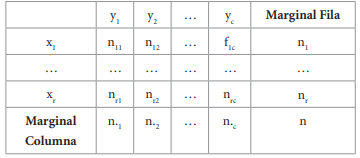
\includegraphics{tabla_corres.png}
    %\caption{Caption}
    \label{tab1}
\end{table}


La frecuencia $n_i_.$ = $\sum_{j=1}^{c}n_i_j$ 
recibe  el  nombre  de  frecuencia marginales de X, y     $n_._j$ = $\sum_{i=1}^{r}n_i_j$ recibe
el nombre de frecuencia marginal de
Y. El valor $n_._.$ = $\sum_{j=1}^{c}\sum_{i=1}^{r}n_i_j$ es el valor
de la frecuencia total de la tabla.
\subsubsection{Dependencia e independencia
en las tablas de correspondencia} 
La independencia o dependencia
entre X y Y se la verifica habitualmente utilizando la $X^2$
 de Pearson, donde
se verifica la hipótesis nula H0
: $X$ y $Y$
son independientes y la hipótesis alternativa $X$ y $Y$ son dependientes, según: valor p=$X^2_(r-1)_(c-1) >= G^2$ para
un nivel de significación la Hipótesis
$H_o$ se rechaza si dicho valor-p es
menor o igual a 0.05. Dónde:

\begin{equation}
G^2 = \sum_{i=1}^{r}\sum_{j=1}^{c}\frac{(n_i_j-e_i_j)^2}{e_i_j} 
\label{eq1}
\end{equation}

Si la hipótesis nula se rechaza,
las variables X y Y son dependientes,
es conveniente saber el tipo de dependencia, esto se logra obteniendo
los residuos tipificados corregidos :
\begin{equation}
r_i_j = \frac{n_i_j-e_i_j}{\sqrt{e_i_j}\sqrt{1-\frac{n_i_.}{n_._.}}}}{\sqrt{1-\frac{n_._j}{n_._.}}}

\end{equation}

\subsubsection{Descomposicion de los valores singulares}

Para matrices rectangulares generales puede conseguirse una descomposición similar a la descomposición espectral de una matriz
simétrica. Como en el caso de matrices cuadradas y simétricas, toda matriz rectangular de dimensiones (r ×
c) y de rango r puede expresarse como
producto de tres matrices, dos con
vectores ortogonales y una diagonal.
La descomposición es
 = UDV’
Donde U es (r × k), D es (k ×
k) y V’ es (c × k), donde k = min{r1,c-1}. La matriz diagonal D contiene las raíces cuadradas de los valores propios no nulos de las matrices
CC’ o C’C , que son positivos. Estos
términos diagonales de D =diag(μ1
,
μ2
, .., μk
) se denominan los valores
singulares de la matriz . La matriz U
contiene en columnas los vectores
propios unidos a valores propios no
nulos de CC’ y V contiene en columnas los vectores propios unidos
a valores propios no nulos de C’C.
Las columnas de U son ortogonales
entre sí y también lo serán las de V.
Los elementos diagonales de D se
denominan los valores singulares de
la matriz A (Daniel, 2002).
Las matrices A y B se calculan a
partir de las expresiones:
$$A=D_r^{\frac{1}{2}}UD$$
$$B=D_c^{\frac{1}{2}}VD$$

Para esta sección de tomaron de la base de datos de mujeres solteras, las siguientes variables:
\begin{itemize}
\item Departamento de Residencia
\item ¿ A lo largo de su vida, en algún lugar público algún(os) hombre(s) conocido(s) o desconocido(s), sin considerar a su (ex) pareja/ (ex) novio, la han humillado o menospreciado (la han hecho sentir menos)?
\end{itemize}

Respecto a la segunda variable de ínteres en esta sección por lo ya definido en el marco teorico se trata de Violencia Psícologica contra las mujeres, en el ámbito social. 

La dos variables son de tipo cualitativa con mas de dos categorias en la variable Departamento. Usando el metodo ya mencianado se puede observar el siguiente grafico resopecto a las relacion de las variables
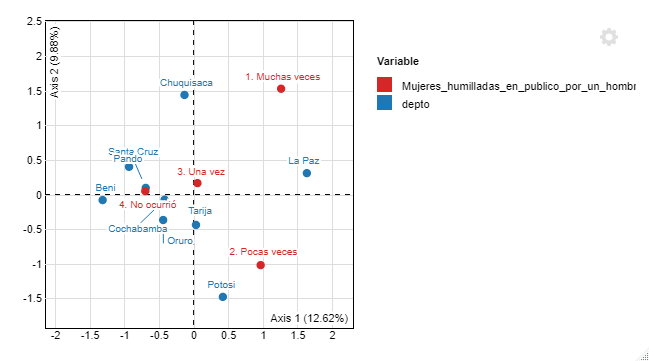
\includegraphics{analisis_corres.png}

\subsection{Clasificación Logit}
La forma funcional del modelo logit es:
$$ y_i = \beta_i + \sum_{i=2}^{k}\beta_i^k X_i^k + \epsilon_i


donde x = (x1,x2,...xk) es el vector de características del hogar,yi* es la variable dependiente que no es observable; lo que se observa es una variable dicotómica definida por: Yi = 1 si Yi*>0 Yi = 0 e. o. c y lo que se estima es la probabilidad de ocurrencia de la variable dependiente:

Prob(Yi)=Prob (Yi*>0)=Prob(εi>-βXi)
Prob(Yi)=1 -F( -βXi),

donde F es la función de distribución acumulativa de e, siendo ei ~N(0,o2), que al ser logística tiene la siguiente forma:



La clasificación de pobre o no pobre se obtiene a partir de la probabilidad estimada  y un punto de corte de esta probabilidad. l + exp(A)

Las medidas más recomendadas para verificar la bondad de ajuste de los modelos Logit y Probit pueden ser el valor de la función de verosimilitud en el máximo valor; el estadístico L que surge de una prueba de homoscedasticidad con distribución X2(p)g.l. (donde p es el número de variables explicativas dentro del modelo). Si este estadístico es mayor que el valor crítico no rechazamos H0, y este modelo es homoscedástico. El coeficiente de determinación pseudo R2 es también una medida de bondad de ajuste que toma en cuenta la restricción del rango de las variables cualitativas.

\subsubsection{Aplicacion del Metodo }
segun la investigacion \autocite{cruz2019factores}, en su articulo que se basa a datos recopilados de caso de feminicidio en Bolivia en los años 2016 y 2017 segun datos proporcionados por la FELCV, las principales armas utilizadas en feminicidios fueron:
\begin{itemize}
    \item arma de fuego
\item arma blanca
\item contusiones
\item lazo 
\item toxicos 
\end{itemize}

La moyoria de estas caracteristicas se encuentran en las variables de nuestra bd_cas,las cuales son,

¿Desde que inició la relación con su (ex) pareja/ (ex) novio, alguna vez él:

\begin{itemize}
    \item  la ha abofeteado, golpeado con las manos o puños?

\item  la ha golpeado con algún objeto?

\item	 la ha pateado?
\item	 la ha tratado de ahorcar o asfixiar?

\item	la ha agredido con cuchillo, navaja, pistola o cualquier otra arma?

\item	le ha disparado con un arma?
 
\end{itemize}

Definiendo " Indicio de Feminicidio'' una variable
\begin{itemize}
    \item Indicios de Feminicidio: por los menos sucedio una ves alguna de las variables ya mencionadas

\end{itemize}
variable de tipo binario
donde " Indicios de Feminicidio'' es un posible indicador de indicios de feminicidio.

\begin{figure}[!htp]
%\centering
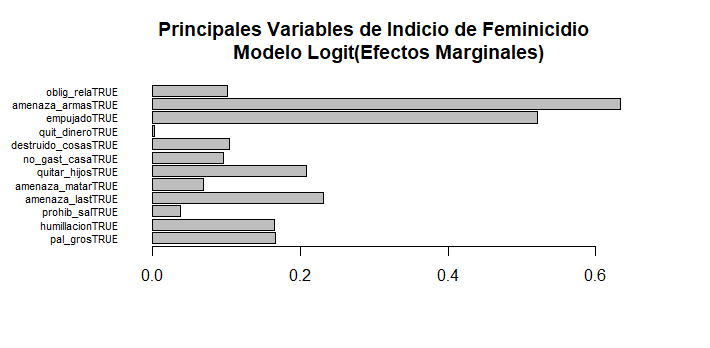
\includegraphics[scale=0.7]{log2.png}
\caption{Modelo Logit}
\label{f1_log}
\end{figure}

Las etiquetas de las variables en la figura \ref{f1_log} son las siguientes:
¿Desde que inició la relación con su (ex) pareja/ (ex) novio, alguna vez él,						

\begin{itemize}
    %\item exige-rela: le ha exigido tener relaciones sexuales aunque usted no quería?
    item oblig-rela:  ha usado la fuerza física para obligarla a tener relaciones sexuales?
    \item amenaza-armas:la ha amenazado con armas (cuchillo, navaja o pistola)?
    \item empujado:  la ha empujado o le ha jalado el cabello?
    \item quit-dinero:  le ha quitado, o se ha adueñado de su dinero?
    \item destruido-cosas:  ha destruido, tirado o escondido sus cosas?
    \item no-gast-casa : aunque tenga dinero no cumple con los gastos del hogar?
    %\item prohib-prop:  le ha prohibido adquirir bienes o propiedades a su nombre?
    \item quitar-hijos:  la ha amenazado con quitarle a sus hijos/as?
    \item amenaza-matar:  la ha amenazado con matarla?
    \item amenaza-last: la ha amenazado con lastimarla ?
    \item prohib-sal: aunque tenga dinero no cumple con los gastos del hogar?
    \item humillacion: la ha avergonzado, menospreciado o humillado?
    \item pal-gros: la ha insultado, se dirigió a usted con palabras groseras o agresivas?
    
\end{itemize}


\subsection{Árboles de Clasificación (CART) }
El método CART uso condiciones basadas en cortes sobre covariables para realizar la clasificación (predicción) de una clase. El proceso de clasificación comienza desde el nodo raíz del árbol; en cada nodo, el proceso verificará si el valor de entrada debe continuar de forma recursiva hacia la sub-rama derecha o izquierda de acuerdo con la condición de división, y se detiene al encontrar cualquier nodo hoja (terminal) del árbol de decisión.

\begin{figure}[!htp]
    \centering
    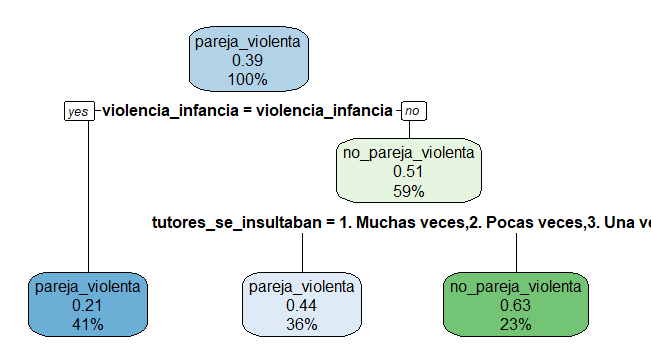
\includegraphics[scale=0.8]{cart.png}
    \caption{Modelo Cart}
    \label{f1_cart}
\end{figure}


\section{Resultados y Análisis}


Un resultado notable referido al analisis de correspondencia , que se pudo realizar, es que se puede evidenciar que, existe con mas intensidad diferentes tipos de Violencia en la región del altiplano de Bolivia y va disminuyendo a medida que la región tiende al oriente como los departamentos de Pando, Beni y Santa Cruz, en las que la Violencia contra las mujeres es muy reducido en comparación con los departamentos de La Paz, Oruro y Potosí.

Con el modelo logit con una acauracidad del 87 por ciento se puede notar que en los hogares de las mujeres encuestadas, en este caso base de datos muejeres casadas se pudo obtener grandes resultados con la intencion de encontrar algunos patrones que puedan evidenciar indicios de Feminicifo en sus respectivos Hogares.  

Con el metodo CART se puede notar que una de las razones del porque existe Violencia contra las mujeres es el hogar donde crecieron sus parejas, para la aplicacion del metodo se utilizo la base de datos de muejeres separadas. Los resultados obtenidos tienen una acuaracidad del 61 por ciento. 

\section{Conclusiones y Recomendaciones}

\subsection{Conclusiones}
Se puede notar solo con los pocos resultados que se pudo obtener se puede evidenciar que uno de los grandes flagelos de nuestra sociedad es la Violencia contra las Mujeres que posteriormente puede llegar a mayores consecuencias como Feminicidios. 

Con los resultados de la encuesta en cuestión se ha podido mostrar que por lo menos 5 de cada 10 mujeres viven o han vivido algún tipo de Violencia en Bolivia.

\subsection{Recomendaciones}
Por la gran cantidad de variables que se cuenta en las bases de datos siendo estas al rededor de 710, no se mostró tan a detalle varios resultados que podrían llegar a ser de gran utilidad. Todo esto con el fin de encontrar indicadores que puedan ayudar a detectar como por ejemplo indicios o comportamientos de Feminicidio.


 

\printbibliography

\end{document}